\documentclass[11pt]{article}
\usepackage[a4paper,margin=1in]{geometry}
\usepackage{amsmath,amssymb}
\usepackage[T1]{fontenc}
\usepackage{lmodern}
\usepackage{microtype}
\usepackage{xcolor}
\usepackage{footnote}
\usepackage{tikz}
\usetikzlibrary{arrows.meta,calc}

\setlength{\parindent}{0pt}
\setlength{\parskip}{0.5em}

\newcommand{\promptbox}[1]{%
  \begin{savenotes}%
  \begingroup\setlength{\fboxsep}{10pt}\noindent
  \colorbox{blue!8}{\parbox{\dimexpr\linewidth-2\fboxsep\relax}{\textbf{Prompt. }#1}}
  \endgroup
  \end{savenotes}%
}
\newcommand{\resultbox}[1]{%
  \begin{savenotes}%
  \begingroup\setlength{\fboxsep}{10pt}\noindent
  \colorbox{purple!8}{\parbox{\dimexpr\linewidth-2\fboxsep\relax}{\textbf{Result. }#1}}
  \endgroup
  \end{savenotes}%
}
\newcommand{\examplebox}[1]{%
  \begin{savenotes}%
  \begingroup\setlength{\fboxsep}{10pt}\noindent
  \colorbox{green!8}{\parbox{\dimexpr\linewidth-2\fboxsep\relax}{\textbf{Example. }#1}}
  \endgroup
  \end{savenotes}%
}

\title{\textbf{Book 1 --- Lecture 2 --- Exercise 5}\\[2mm]
\large Derivatives of \(\sin\), \(\cos\), \(\exp\), and \(\ln\)}
\author{}
\date{}

\begin{document}
\maketitle

\promptbox{Prove each of the formulas:
\[
\frac{d}{dt}\sin(t)=\cos(t),\qquad
\frac{d}{dt}\cos(t)=-\sin(t),\qquad
\frac{d}{dt}e^{t}=e^{t},\qquad
\frac{d}{dt}\ln(t)=\frac{1}{t}.
\]
Hint: Look up trigonometric identities and limit properties in a reference
book.\footnote{All limits below are one-sided at domain boundaries where needed
(\(t>0\) for \(\ln t\)). Angles are in radians.}}

\section*{Two standard limits}
The sine and cosine proofs use
\[
\lim_{h\to 0}\frac{\sin h}{h}=1
\qquad\text{and}\qquad
\lim_{h\to 0}\frac{\cos h-1}{h}=0.
\]
The second follows from the first via the identity \(1-\cos h=2\sin^2(h/2)\):
\[
\frac{1-\cos h}{h}
=\frac{2\sin^2(h/2)}{h}
=\underbrace{\left(\frac{\sin(h/2)}{h/2}\right)^2}_{\to\,1}\cdot\frac{h}{2}\to 0,
\]
hence \(\dfrac{\cos h-1}{h}\to 0\).

\paragraph{Picture (small-angle limits).}
On the unit circle, a small central angle \(h\) (radians) cuts off an arc of length
\(h\) and a vertical segment of length \(\sin h\). For \(h\to 0^{+}\), arc and
segment nearly coincide, so \(\sin h/h\to 1\). The point on the circle lies at
\((\cos h,\sin h)\), so the horizontal gap \(1-\cos h\) is much smaller than \(h\);
that is the geometric content of \((\cos h-1)/h\to 0\).

\begin{center}
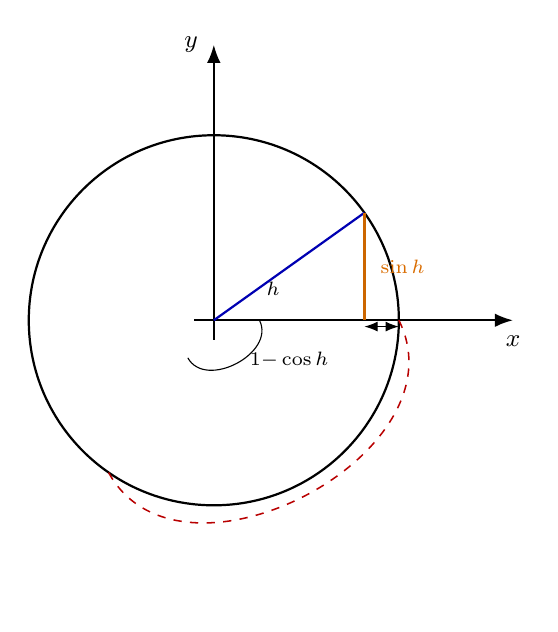
\begin{tikzpicture}[>=Latex, thick, trig format=rad, x=1cm, y=1cm]
  \def\R{2.35}
  \def\h{0.62}
  \pgfmathsetmacro{\hdeg}{deg(\h)}
  \coordinate (O) at (0,0);
  \coordinate (A) at (\R,0);
  \coordinate (P) at ({\R*cos(\h)},{\R*sin(\h)});
  \draw[->] (-0.25,0) -- (\R+1.45,0) node[below=2pt, font=\small]{$x$};
  \draw[->] (0,-0.25) -- (0,\R+1.15) node[left=2pt, font=\small]{$y$};
  \draw (O) circle (\R);
  \draw[blue!70!black] (O) -- (P);
  \draw[orange!80!black] (P) -- ({\R*cos(\h)},0);
  \draw[red!72!black, dashed, line width=0.55pt]
    (A) arc[start angle=0, end angle=\hdeg, radius=\R];
  \draw[thin] (0.58,0) arc[start angle=0, end angle=\hdeg, radius=0.58];
  \node[font=\scriptsize, anchor=south west, inner sep=1pt] at (0.62,0.26) {$h$};
  \node[font=\scriptsize, orange!85!black, anchor=west, inner sep=2pt]
    at ({\R*cos(\h)+0.12},{\R*sin(\h)/2}) {$\sin h$};
  \node[font=\scriptsize, anchor=north, inner sep=2pt] at ({\R*cos(\h)/2},{-0.32}) {$1{-}\cos h$};
  \draw[<->, thin] ({\R*cos(\h)},-0.08) -- (\R,-0.08);
\end{tikzpicture}\\[0.5em]
{\small Angle exaggerated for readability; the limits use \(h\to 0\).}
\end{center}

\section*{\(\dfrac{d}{dt}\sin(t)=\cos(t)\)}
For \(h\neq 0\), the addition formula \(\sin(t+h)=\sin t\cos h+\cos t\sin h\) gives
\[
\frac{\sin(t+h)-\sin(t)}{h}
=\sin t\,\frac{\cos h-1}{h}+\cos t\,\frac{\sin h}{h}.
\]
Let \(h\to 0\). The first term \(\to 0\) and the second \(\to\cos t\), so
\(\dfrac{d}{dt}\sin(t)=\cos(t)\).

\paragraph{Picture (sine).}
The Newton quotient \(\bigl(\sin(t{+}h)-\sin(t)\bigr)/h\) is the slope of the chord
joining two points on \(y=\sin t\). As \(h\to 0\), that chord approaches the tangent
line, whose slope is \(\cos t\).

\begin{center}
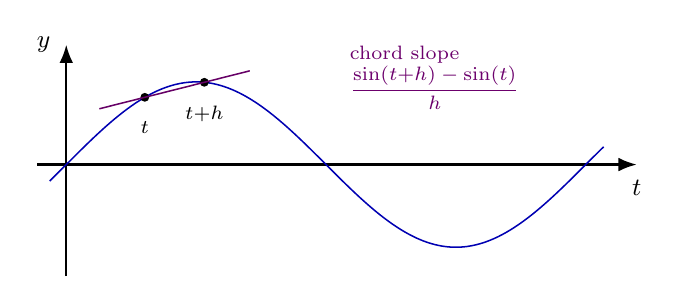
\begin{tikzpicture}[>=Latex, thick, trig format=rad, x=1.05cm, y=1.05cm]
  \def\tzero{0.95}
  \def\hh{0.72}
  \pgfmathsetmacro{\tone}{\tzero+\hh}
  \pgfmathsetmacro{\ys}{sin(\tzero)}
  \pgfmathsetmacro{\ye}{sin(\tone)}
  \pgfmathsetmacro{\slope}{(sin(\tone)-sin(\tzero))/\hh}
  \draw[->] (-0.35,0) -- (6.9,0) node[below=2pt, font=\small]{$t$};
  \draw[->] (0,-1.35) -- (0,1.45) node[left=2pt, font=\small]{$y$};
  \draw[blue!70!black, smooth, domain=-0.2:6.5, samples=90, line width=0.55pt]
    plot (\x, {sin(\x)});
  \coordinate (T0) at (\tzero,\ys);
  \coordinate (T1) at (\tone,\ye);
  \fill (T0) circle (1.6pt) node[below=5pt, font=\scriptsize]{$t$};
  \fill (T1) circle (1.6pt) node[below=5pt, font=\scriptsize]{$t{+}h$};
  \draw[violet!80!black, line width=0.55pt] ($(T0)+(-0.55,-0.55*\slope)$) -- ($(T1)+(0.55,0.55*\slope)$);
  \node[font=\scriptsize, violet!85!black, anchor=west, inner sep=2pt, align=left]
    at (3.35,1.05) {chord slope\\$\displaystyle\frac{\sin(t{+}h)-\sin(t)}{h}$};
\end{tikzpicture}\\[0.5em]
{\small The illustration fixes a sample \(t,h\); the proof is the limit \(h\to 0\).}
\end{center}

\section*{\(\dfrac{d}{dt}\cos(t)=-\sin(t)\)}
Using \(\cos(t+h)=\cos t\cos h-\sin t\sin h\),
\[
\frac{\cos(t+h)-\cos(t)}{h}
=\cos t\,\frac{\cos h-1}{h}-\sin t\,\frac{\sin h}{h}
\longrightarrow -\sin t.
\]

\paragraph{Picture (cosine).}
The same chord idea applies to \(y=\cos t\). Here the chord slope tends to
\(-\sin t\) (downhill where \(\sin t>0\)).

\begin{center}
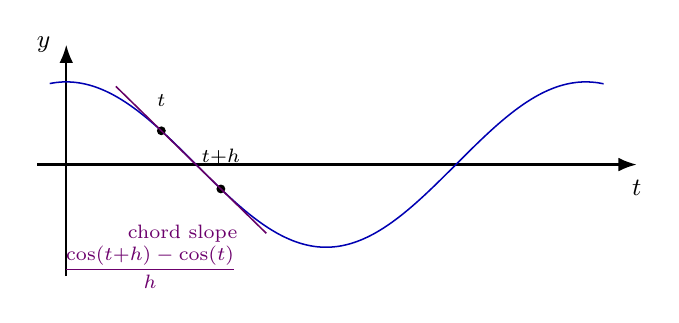
\begin{tikzpicture}[>=Latex, thick, trig format=rad, x=1.05cm, y=1.05cm]
  \def\tzero{1.15}
  \def\hh{0.72}
  \pgfmathsetmacro{\tone}{\tzero+\hh}
  \pgfmathsetmacro{\ys}{cos(\tzero)}
  \pgfmathsetmacro{\ye}{cos(\tone)}
  \pgfmathsetmacro{\slope}{(cos(\tone)-cos(\tzero))/\hh}
  \draw[->] (-0.35,0) -- (6.9,0) node[below=2pt, font=\small]{$t$};
  \draw[->] (0,-1.35) -- (0,1.45) node[left=2pt, font=\small]{$y$};
  \draw[blue!70!black, smooth, domain=-0.2:6.5, samples=90, line width=0.55pt]
    plot (\x, {cos(\x)});
  \coordinate (T0) at (\tzero,\ys);
  \coordinate (T1) at (\tone,\ye);
  \fill (T0) circle (1.6pt) node[above=5pt, font=\scriptsize]{$t$};
  \fill (T1) circle (1.6pt) node[above=5pt, font=\scriptsize]{$t{+}h$};
  \draw[violet!80!black, line width=0.55pt] ($(T0)+(-0.55,-0.55*\slope)$) -- ($(T1)+(0.55,0.55*\slope)$);
  \node[font=\scriptsize, violet!85!black, anchor=east, inner sep=2pt, align=right]
    at (2.15,-1.12) {chord slope\\$\displaystyle\frac{\cos(t{+}h)-\cos(t)}{h}$};
\end{tikzpicture}\\[0.5em]
{\small Again, a fixed sample \((t,h)\) for drawing; the derivative is the limit.}
\end{center}

\section*{\(\dfrac{d}{dt}e^{t}=e^{t}\)}
For every \(h\neq 0\),
\[
\frac{e^{t+h}-e^{t}}{h}=e^{t}\cdot\frac{e^{h}-1}{h}.
\]
It suffices to show \(\displaystyle\lim_{h\to 0}\frac{e^{h}-1}{h}=1\).\footnote{Many
texts define \(e^{x}\) first (series, integral, or limit) and derive this limit; the
lecture hint points to a reference for whichever route your edition uses. One common
route: with \(e^{x}=\sum_{n=0}^{\infty}x^{n}/n!\), one has
\(e^{h}-1=h+h^{2}/2!+\cdots=h(1+O(h))\), so \((e^{h}-1)/h\to 1\).}
Then \(\dfrac{d}{dt}e^{t}=e^{t}\cdot 1=e^{t}\).

\paragraph{Picture (exponential).}
The graph \(y=e^{t}\) is self-similar in vertical scale: shifting \(t\) by \(h\)
multiplies heights by \(e^{h}\). Thus
\(\bigl(e^{t+h}-e^{t}\bigr)/h=e^{t}\cdot (e^{h}-1)/h\): the secant slope at height
\(e^{t}\) is \(e^{t}\) times the normalized slope \((e^{h}-1)/h\) through \((0,1)\).

\begin{center}
\begin{tikzpicture}[>=Latex, thick, x=1.45cm, y=0.85cm]
  \def\ta{0.25}
  \def\hb{0.85}
  \pgfmathsetmacro{\tb}{\ta+\hb}
  \pgfmathsetmacro{\ya}{exp(\ta)}
  \pgfmathsetmacro{\yb}{exp(\tb)}
  \pgfmathsetmacro{\slope}{(\yb-\ya)/\hb}
  \draw[->] (-0.25,0) -- (2.85,0) node[below=2pt, font=\small]{$t$};
  \draw[->] (0,-0.25) -- (0,6.35) node[left=2pt, font=\small]{$y$};
  \draw[blue!70!black, smooth, domain=-0.12:2.35, samples=50, line width=0.55pt]
    plot (\x, {exp(\x)});
  \coordinate (A) at (\ta,\ya);
  \coordinate (B) at (\tb,\yb);
  \fill (A) circle (1.6pt) node[left=4pt, font=\scriptsize]{$t$};
  \fill (B) circle (1.6pt) node[right=3pt, font=\scriptsize]{$t{+}h$};
  \draw[violet!80!black, line width=0.55pt] ($(A)+(-0.22,-0.22*\slope)$) -- ($(B)+(0.22,0.22*\slope)$);
  \draw[dashed, gray!60] (0,1) -- (2.35,1);
  \node[font=\scriptsize, anchor=east, inner sep=2pt] at (-0.1,1) {$1$};
  \node[font=\scriptsize, violet!85!black, anchor=west, align=left, inner sep=2pt]
    at (1.55,5.35) {secant slope\\$\displaystyle\frac{e^{t+h}-e^{t}}{h}$};
\end{tikzpicture}\\[0.5em]
{\small Vertical stretch factor \(e^{t}\) links this secant to \((e^{h}-1)/h\) at the reference point \((0,1)\).}
\end{center}

\section*{\(\dfrac{d}{dt}\ln(t)=\dfrac{1}{t}\) for \(t>0\)}
Fix \(t>0\) and take \(h\neq 0\) small enough that \(t+h>0\). Then
\[
\frac{\ln(t+h)-\ln(t)}{h}
=\frac{1}{h}\ln\!\left(1+\frac{h}{t}\right)
=\frac{1}{t}\cdot\frac{\ln(1+u)}{u},
\qquad u=\frac{h}{t}.
\]
As \(h\to 0\), also \(u\to 0\). If \(v=\ln(1+u)\), then \(u=e^{v}-1\) and \(v\to 0\)
as \(u\to 0\), and
\[
\frac{\ln(1+u)}{u}=\frac{v}{e^{v}-1}
=\left(\frac{e^{v}-1}{v}\right)^{-1}\longrightarrow 1
\]
using the same exponential limit \(\dfrac{e^{v}-1}{v}\to 1\) as above. Therefore the
Newton quotient tends to \(\dfrac{1}{t}\).

\paragraph{Picture (logarithm).}
On \(y=\ln t\), a step \(\Delta t=h\) produces a rise \(\ln(t{+}h)-\ln(t)\). Writing
\(u=h/t\), the relative step along the horizontal axis is \(u\); the quotient
\(\ln(1+u)/u\) is the slope of the chord from \((1,0)\) to \((1{+}u,\ln(1{+}u))\) in a
\emph{normalized} picture, and it tends to \(1\) as \(u\to 0\). Rescaling by \(1/t\)
gives slope \(1/t\) at \(t\).

\begin{center}
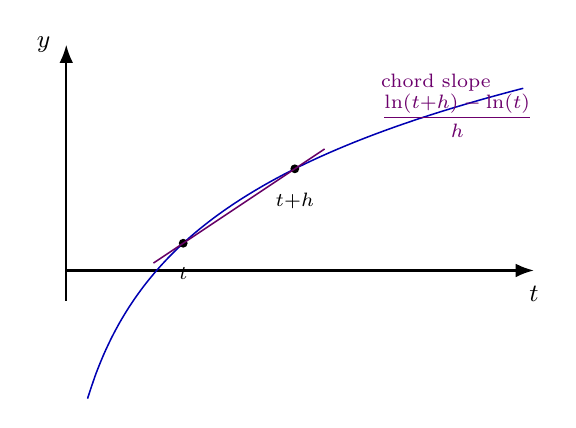
\begin{tikzpicture}[>=Latex, thick, x=1.35cm, y=1.55cm]
  \def\tt{1.25}
  \def\hd{1.05}
  \pgfmathsetmacro{\tp}{\tt+\hd}
  \pgfmathsetmacro{\yl}{ln(\tt)}
  \pgfmathsetmacro{\yr}{ln(\tp)}
  \pgfmathsetmacro{\slope}{(\yr-\yl)/\hd}
  \draw[->] (0.15,0) -- (4.55,0) node[below=2pt, font=\small]{$t$};
  \draw[->] (0.15,-0.25) -- (0.15,1.85) node[left=2pt, font=\small]{$y$};
  \draw[blue!70!black, smooth, domain=0.35:4.45, samples=55, line width=0.55pt]
    plot (\x, {ln(\x)});
  \coordinate (L0) at (\tt,\yl);
  \coordinate (L1) at (\tp,\yr);
  \fill (L0) circle (1.6pt) node[below=5pt, font=\scriptsize]{$t$};
  \fill (L1) circle (1.6pt) node[below=5pt, font=\scriptsize]{$t{+}h$};
  \draw[violet!80!black, line width=0.55pt] ($(L0)+(-0.28,-0.28*\slope)$) -- ($(L1)+(0.28,0.28*\slope)$);
  \node[font=\scriptsize, violet!85!black, anchor=west, align=left, inner sep=2pt]
    at (3.05,1.35) {chord slope\\$\displaystyle\frac{\ln(t{+}h)-\ln(t)}{h}$};
\end{tikzpicture}\\[0.5em]
{\small Domain \(t>0\); the algebra rewrites this slope as \(\dfrac{1}{t}\cdot\dfrac{\ln(1+u)}{u}\) with \(u=h/t\).}
\end{center}

\resultbox{For all real \(t\) (in radians),
\[
\frac{d}{dt}\sin(t)=\cos(t),\qquad \frac{d}{dt}\cos(t)=-\sin(t).
\]
For all real \(t\), \(\dfrac{d}{dt}e^{t}=e^{t}\). For \(t>0\),
\(\dfrac{d}{dt}\ln(t)=\dfrac{1}{t}\).}

\examplebox{Check at \(t=0\): \(\cos'(0)=-\sin(0)=0\); \(\dfrac{d}{dt}\ln(t)\) is not
defined at \(t=0\) because \(\ln\) is undefined there.}

\end{document}
